%!TEX root = ../../thesis.tex
	Acknowledgment: Florian, Akitoshi
	\section{Introduction}
		As seen in Chapter \ref{section:real_complexity} many important operators 
		on real functions have been shown to be computationally hard.
		On the other hand, numerical scientists can quickly compute maxima or anti-derivatives of functions.
		To analyze this mismatch one should ask the follwing questions
		\begin{enumerate}
			\item What subset of real functions is usually considered in numerical analysis?
			\item Are there implicit assumptions made about the functions, that allow faster computations? 
		\end{enumerate}
		One class of functions that has been considered in computable analysis is the analytic functions.
		Although not at all sufficent as the class of functions considered interesting for numerical analysis, 
		many computations become tractable when one restricts the attention to analytic functions.
		\begin{definition}
			For $z \in \CC$ and $r \in \RR, r > 0$, let $B(z,r) := \{ x \in \CC \,\, | x - z | < r\}$. \\
			A function $f: D \to \CC$ with $D \subseteq CC$ is called \textbf{analytic} if for every $x_0 \in D$ 
			the function given by the Taylor-series around $x_0$ converges to $f(x)$ for every $x$ in a neighborhood of 
			$x_0$. 
			That is, for every $x_0 \in \D$ there is a $\varepsilon > 0$, such that for all $x \in B(x_0, \varepsilon)$ and for 
			$$ T(x) := \sum_{n=0}^{\infty} \frac{f^{(n)}(x_0)}{n!}(x-x_0)^n  \text{, } T(x) \rightarrow f(x)$$.
			The set of functions analytic on $D$ is denoted as $C^\infty(D)$. \\
			The coefficients of the Taylor expansion is denoted by the series $(a_n)_{n \in \NN}$, i.e. 
			$$ a_n = \frac{f^{(n)}(x_0)}{n!}. $$    
			For the sake of simplicity, it will w.l.o.g. be assumed that $x_0 = 0$  and $D = [0,1]$ if not stated otherwise.
		\end{definition}
		Note: The above definition can be easily generalized to higher dimension. \\
		Some properties of analytic functions...
		The complexity of analytic functions is much better then for the general case.
		\begin{theorem}[Pour-El, Richards, Ko, Friedman, Müller] 
			The following are equivalent
			\begin{enumerate}
				\item $f$ is computable 
				\item The series $(a_n)_{n \in \NN}$ is computable. 
 			\end{enumerate}
 			The equivalence also holds, when computable is replaced by polynomial time computable.
		\end{theorem}
		From that it follows
		\begin{corollary}
			If $f$ is polynomial time computable the following functions are
			\begin{enumerate}
				\item $I: [0,1] \to \RR$, $I(x) = \int_0^x f(t) dt$
				\item $D: [0,1] \to \RR$, $D(x) = f'(x)$ 
			\end{enumerate}
			\begin{proof}
				Taylor-series
			\end{proof}
		\end{corollary}
		Even tough the above results are nice, those theorems are non-uniform.
		The theorems only say that, when $f$ is polynomial time computable, then there exists 
		a polynomial time computable coefficient sequence and if there is a polynomial time computable sequence, then
		there is some algorithm that can compute the series in polynomial time.
		In no way, however, do they say, how to compute the sequence from a given representation of the function and vice versa.
		In fact the following theorems show, that this is not a problem of those theorems, but it's inherently impossible to do this.
		\begin{theorem}[M\"uller \cite{Mue}]
			Let $f$ given as in ... then the operator $f \to (a_n)_{n \in \NN}$ computing the Taylor series around $0$ (or any other point) is not computable.
		\end{theorem} 
		\begin{theorem}[M\"uller \cite{Mue}]
			Let $(a_n)_{n \in \NN}$ be the series expansion around $0$ for some $f \in C^\omega(D)$.\\
			The evaluation operator $((a_n)_{n \in \NN}, x) \to f(x)$ that, given a series and a point, computes the value of the corresponding function at that point, is not computable.
			\begin{proof}
				One does not know how many coefficients needed...
			\end{proof}
		\end{theorem} 

	\section{Representation of Analytic Functions}
	 As seen in the previous section, the information given by the series expansion is not enough to represent an analytic function.
	 However, by enriching the information by some finite discrete parameters, the translation between Taylor-series and function representation can be made uniform.
	 In particular the following two representation for analytic functions are useful
	 \begin{definition}\label{def:series_name_ball}
	 	A \textbf{series-name} $\rho_s$ of $f \in C^\omega(\overline{B_1(0)})$ is a triple $((a_n)_{n \in \NN}, k, A)$ where 
	 	\begin{enumerate}
	 		\item $(a_n)_{n \in \NN}$ is the series expansion of $f$ around $0$
	 		\item $\sqrt[k]{2} \leq R$ 
	 		\item $|a_j|r^j \leq A$ for all $j \in \NN$
	 	\end{enumerate}
	 	where $R = (\limsup |a_j|^{\frac{1}{j}})^{-1}$ denotes the radius of convergence of the series.
	 \end{definition}
	 Those two additional parameters can be used to make a tail estimate 
	 \begin{equation}\label{eqn:tail_estimate}
	  \left | \sum_{n \geq N} a_nx^n \right | \leq A \frac{(|z|/r)^N}{1-|z|/r}
	 \end{equation}
	 A name as in Definition \ref{def:series_name_ball} can be found by choosing any appropriate $k$ (note that the radius of convergence is always bigger than $1$) and choosing $A$ as an upper bound of $f$ extended to $\overline{B_{\sqrt[k]{2}}(0)}$. 
	 \begin{definition}
	 	A \textbf{function-name} $\rho_f$ of $f \in C^\omega(\overline{B_1(0)})$ is a triple $(f, l, B)$ such that
		B is an upper bound of $f$ on $\overline{B_{\sqrt[l]{2}}(0)}$.
	 \end{definition}
	 \begin{theorem}\cite{Kaw}\label{thm:representation_conversion}
	 	The mapping between $\rho_s$-name and $\rho_f$-names is computable in time polynomial in 
	 	$n+k+\log(A)$ and the inverse mapping is computable in time polynomial in $n+l+\log(B)$ 
	 \end{theorem}
	 \begin{proof}
	 	To compute a function name from a series name it only has to be shown that evaluation...

	 	To compute a series name from a function name, one has to compute the coefficients of the series expansion from a function name, i.e. from the function and the parameters $l$ and $B$.
	 	In \cite{Mue} M\"uller describes an algorithm for this task.
	 	To approximate the coefficient $a_k$ with precision at least $2^{-n}$ $f$ is approximated by the Lagrangian interpolation
	 	polynomial
	 	\begin{equation}\label{eqn:interpolation_polynomial}
	 		P_m(x)  :=  \sum_{i=0}^{2m} f(x_i) \cdot L_{m,i}(x) 
	 	\end{equation}
	 	where
	 	\begin{eqnarray*}
	 		x_i & = & (i-m) \cdot h , h \in \RR, h > 0 \\
	 		L_{m,i}(x) & = & \prod_{i \neq j} \frac{x-x_j}{x_i-x_j} 
	 	\end{eqnarray*}
	 	Differentiating Equation \ref{eqn:interpolation_polynomial} $k$ times yields
	 	\begin{equation}\label{eqn:interpolation_polynomial_diff}
	 		P_m^k(0)  :=  \sum_{i=0}^{2m} f(x_i) \cdot L_{m,i}^{(k)}(x) 
	 	\end{equation}
	 	Let $\sigma = \lceil \log_2 B \rceil + 1$

	 	It can then be shown that if $f$ is evaluated on $2k+1$ points from the 
	 	real interval $\{x \in \R \,|\, |x| \leq \frac{1}{2}\}$ with precision $2n+15k+\sigma+6$ 
	 	then $a_k$ can be approximated by the above procedure with error less than $2^{-n}$ in 
	 	$O((k+1)\cdot \M(n+k+\sigma) + k^2 \M (k \log k)$

	 \end{proof}
	 Note that the above translation becomes fully polynomial time when in the representations $k$ resp. $l$ are required to be encoded in unary, while $A$ resp. $B$ are given in binary.
	 Thus, from now on the term polynomial time computable will be used when referring to running time bounds as in Theorem \ref{thm:representation_conversion}.
	 \begin{theorem}\label{thm:polytime_on_ball}
	 	The following is polynomial time computable when given $\rho_s$ or $\rho_f$ names for the input functions.
	 	\begin{enumerate}
	 		\item Evaluation $(f,z) \to f(z)$
	 		\item Addition $(f_1, f_2) \to f_1 + f_2$
	 		\item Multiplication $(f_1, f_2) \to f_1 \cdot f_2$
	 		\item $d$-fold Differentiation $(f,d) \to f^{(d)}$ where $d$ is given as unary
	 		\item $d$-fold Anti-differentiation $(f,d) \to \int \dots \int f$ where $d$ is given in unary
	 		\item Parametric maximization
	 	\end{enumerate}
	 	\begin{proof}(Sketch)
	 		Evaluation follows from \ref{thm:representation_conversion}. \\
	 		Except for parametric maximization the transformation of the Taylor series is obvious (e.g. for addition, just add the coefficients).
	 		It remains to show how to compute the new parameters $A'$ and $k'$. 
	 	\end{proof}
	 \end{theorem}
	Now consider functions analytic on some other domain, e.g. on the real line $[0,1]$.
	Such functions can be represented by a finite number of powerseries covering the domain. 
	That leads to the following representation
	\begin{definition}\label{def:series_name_rect}
		A \textbf{series-name} for a function $f \in C^\omega([0,1])$ is a 5-tuple $(M, (x_m), (a_{n, j}), k, A)$ where $M \in \NN$
		$1 \leq j \leq M$, $n \in \NN$, $x_m \in [0,1]$ and it holds
		\begin{enumerate}
			\item $[0,1] \subseteq \bigcup_{m=1}^M [x_m - \frac{i}{4k}, x_m + \frac{1}{4k}]$
			\item $(a_{n,i})_{n \in \NN}$ is the series expansion of $f$ around $x_0 + \frac{i}{4k}$
			\item $|a_{n,i}| \leq Ak^n$ for all $n \in N$, $1 \leq i \leq M$
		\end{enumerate}
	\end{definition}
	A function name as in Definition \ref{def:function_name_ball} can also be defined
	\begin{definition}
		Let $R_l := [-\frac{1}{l}, 1+frac{1}{l}] \times [-\frac{1}{l}, frac{1}{l}]$ the closed rectangle around $[-1,1]$ 
		with distance $\frac{1}{l}$ around the line $[0,1]$.
		A \textbf{function-name} for a function $f \in C^\omega([0,1])$ is a 3-tuple $(f|_{[-1,1]}, B, l)$ with $B, l \in \NN$ such that 
		\begin{enumerate}
			\item $f \in C^\omega(R_l)$
			\item $B$ is an upper bound for $f$ on $R_l$
		\end{enumerate}
		Again, $l$ is coded in unary and $B$ in binary.
	\end{definition}
	Again it can be shown that the two representations are polynomial time equivalent, and that the equivalent to
	Theorem \ref{thm:polytime_on_ball} holds.
	\section{Analytic Continuation}
		One problem with the representation in Definition \ref{def:series_name_rect} is that when thinking of this representation as an interface for a datatype, it is very cumbersome for the user to provide all the information needed. 
		One has to give enough Taylor series to cover the whole interval.
		As said before, there is no real gain of information by providing all those series.
		The analytic function is uniquely defined by the Taylor series around a single point.
		Thus, one would like to have something like the following representation
		\begin{definition}
			A \textbf{single series name} for $f \in C^\omega([0,1])$ is a quadruple $(x_0, (a_n)_{n \in \NN}, k, A)$ such that
			\begin{enumerate}
				\item $(a_n)_{n \in \NN}$ is the series expansion of $x$ around $x_0$
				\item $A$ and $k$ are such that $| a_m | \leq Ak^m$ 
			\end{enumerate}
		\end{definition}
		A series name can be computed from a single series name by computing the series expansion on another point on the domain and then iterating this process until the series cover $[0,1]$ (see Figure \ref{fig}).
		Since the parameters $A$ and $k$ are such that they hold on the entire rectangle, 
		the new series will be valid on a ball with the same radius as the original series, effectly extending the domain.
		The series can be computed either by applying the algorithm from the proof of Theorem \ref{thm:representation_conversion} or by directly computing the derivatives at an other point using Theorem \ref{thm:polytime_on_ball}.
		Note however, that iterating this process will break the polynomial time computability, as will be shown in the next
		section.
	\section{Complexity Analysis}
		The previous section gave an overview of the representations and how they can be used to yield efficient 
		operations on analytic functions, where efficient means polynomial time computable.
		Since for practical applications polynomial time computability is too coarse a measure for efficiency, 
		in this section a more refined analysis on the algorithms is done, to establish time bounds in terms of $O$-notation.
		Most of this was already done in \cite{mypaper}.
		Of course, the overall running time will depend on the running time $T(a_m, n)$ that is needed to 
		compute the coefficient $a_m$ with error less than $2^{-m}$.
		\begin{theorem}
			Given a series name of $f \in C^\omega(D)$.
			To evaluate $f$ with error less than $2^{-n}$ 
			$$N = k(n+\lceil log_2(log_2 (e^2) kA \rceil)$$
			coefficients of the Taylor series are sufficent. \\
			This yields evaluation computable in time 
			$$ O(N\M(N)+N \cdot T(a_N, n+log_2(N)+1)) $$ 
		\end{theorem}

		\begin{theorem}
			Computing the $m$-th coefficient of the series for the $d$-fold derivative can be done
			$$ O(T(a_{m+d}, n+d\log_2(d+m)))+d\M(d \log_2 (d+m)+n)) $$
		\end{theorem}

		\begin{theorem}
			Given a series name of $f \in C^\omega(D)$, the number of coefficients of the series of the $d-fold$ derivative computed from $f$ as in Theorem \ref{thm:polytime_on_ball} needed to evaluate this derivative, is given by 
			$$N_d = k\left(n+\lceil log_2(log_2 (e^4) kA \rceil+\left \lceil d\left(\log_2(d)+\log_2(\log_2(e)k+1)-\frac{1}{k}\right)\right\rceil\right).$$
			Thus, evaluating the $d$-fold derivative of $f$ is possible in time bound by
			$$ O(N_d\M(N)+N_d \cdot T(a_{N_d+d}, n+d\log_2(d+N_d)))+d\M(d \log_2 (d+N_d)+n) $$ 
		\end{theorem}
		For computing the $m$-th coefficient of a Taylor series around some point the $m-th$ derivative 
		has to be divided by $m!$. This division reduces the needed precision leading to 
		$$N_{coeff}(m) = 2k\left( n+\lceil log_2(\log_2 (e^4) kA) + m \log_2(log_2(e)k+1)\rceil \right)$$
		as the number of coefficients that are needed to compute the $m-th$ coefficients of the Taylor series 
		around another point. 
		For stepwise analytic continuation it is necessary to iterate the process of differentiating.
		For example, using the single series name when one wants to evaluate the function at a point $x$
		that is not inside the ball of the given series, analytic continuation has to be applied until a series
		containing $x$.
		Assume for a computation the coefficents up to $N$ of the last series is needed. 
		The previous results lead to the recurrence relation
		relation 
		\begin{eqnarray*}
			N^{(0)} &=& N \\
			N^{(l+1)} &=& 2k\left( n+\lceil log_2(\log_2 (e^4) kA) + N^{(l)} \log_2(log_2(e)k+1)\rceil \right)
		\end{eqnarray*}
		leading to
		\begin{theorem}
			Applying analytic continuation $l$ times, to compute $N$ coefficients of the last series 
			\begin{equation}
				N^{(l)} = O((2k \log_2 (\log_2 (e)k +1))^lN) 
			\end{equation}
			coefficients of the original series are needed.
		\end{theorem}
		The above leads to a running bound for evaluating using $l$-times iterated analytic continuation.
		\begin{theorem}
			The running time of evaluating the $l$ times iterated series is bounded by
			\begin{equation}
				 O(l(N^{(l)})^2\M(N^{(l)})+N^{(l)}T(a_{N(l)}, l N^{(l)}\log_2(N^{(l)}))) 
			\end{equation}
		\end{theorem}
	\section{Implementation}
		\irram was used as a framework to implement the ideas in the previous section.
		The goal was to add user friendly classes for analytic functions to \irram.
		In particular two classes were created for this purpose.

		The class \baana is a basic class for analytic functions on 
		a closed disc with rational radius around $0$, inspired by Definition \ref{def:series_name_ball}.

		The class \anarect is a class for functions analytic on an arbitrary real interval $[a,b]$, 
		inspired by Definitions \ref{def:series_name_ball} and \label{def:series_name_rect}.

		Both classes provide a common set of operators and methods, in particular
		\begin{enumerate}
			\item It is possible to add, multiply and subtract two objects using the overloaded operators $+$, $*$, $-$.
			\item It is possible to evaluate the function at $x \in D$ using the overloaded operator $()$
			\item There is a function \code{differentiate (unsigned int n)} to get a new object representing the $d$-th derivative of the analytic function.
			\item There is a function \code{integrate (unsigned int n)} to get a new object representing the $d$-th anti-derivative of the analytic function.
			\item It is possible to get the coefficients of the underlying Taylor series.
		\end{enumerate}

		The implementation heavily uses new features introduced with the \ccx standard...

	\section{Class Overview}
		In addition to the two classes for analytic functions, several helper classes were implemented.
		The implementation tried to stay as close as possible to the interfaces given in the theory section.

		Classes were implemented with generic types using Templates, whenever it made sense.

 		There are two types of classes, classes for representations and classes working on those representation.

		The following classes exist
		
		\subsection{\poly} 
			\textbf{\code{POLY<coeff\_type>}} is a class template for polynomials of a generic coefficient type. 
			The class for the coefficient type should have implementations of the \code{*} and \code{+} operators
			and it should be possible to cast $0$ to \code{<coeff\_type>}.

			The following has been implemented for \poly
			\begin{enumerate}
				\item Constructor from a \code{vector<coeff\_type>} and default constructor (constant zero polynomial).
				\item Copy constructor \code{POLY(const POLY<coeff\_type>\& P)} and Copy assignment constructor \code{POLY\& operator = (const POLY<coeff\_type>\& P)}.
				\item Methods \code{get\_degree()} and \code{get\_coeff(const unsigned int n)} returning the degree and a specific coefficient.
				\item Addition, Subtraction, Multiplication and Scalar Multiplication via the overloaded operators \code{+}, \code{-}, 
				\code{*}, \code{+=}, \code{*=}.
				\item Evaluation via the overloaded operator \code{()}.
				\item symbolic differentiation and integration via the functions \code{void diff(unsigned int)} and \code{void integrate(unsigned int n)}.
				\item A function \code{void rwrite(const POLY<coeff\_type>\& P, int precision)} that outputs the polynomial
				in the form $a_n*X^n+ \dots a_n*X + a_0$ where the real numbers $a_0, \dots, a_n$ are written with the number of decimals given by the parameter \code{precision}.
			\end{enumerate}
			All methods were implemented in the most straight forward way. (Evaluation should be Horner Scheme?)
		\subsection{FUNC}
			\textbf{\func} A class for functions. 
			Works on a a representaton called \code{rep\_rho\_D}.
		\subsection{\powerseries}
			\textbf{\code{POWERSERIES<coeff\_type>}} is a class template for power series of a generic coefficient type, 
			i.e. a (symbolic) series of the form $ \sum_{i=0}^\infty a_n \cdot x^n$.
			
			The series itself is given as a \code{FUNC<coeff\_type(unsigned\ int)>}, i.e. a function from the integers to \code{coeff\_type}. Note, that hereby the maximal number of coefficients is limited by the size of \code{unsigned int}, 
			but the limit is large enough to have no practical relevance.   
			A powerseries works on a representation called \code{rep\_rho\_dy\_omega}. 

		

		The class \textbf{\baana} has two different representations: 
		\code{rep\_pi}, the representation by a power series, and \code{rep\_rho\_D\_refined}, the represention as a function.

		The class \textbf{\anarect} also has two different representations, 
		a function representation \code{rep\_fun} and a series representation calles \code{rep\_ana\_rect}.
	\section{Usage}

	\section{Evaluation}
		Evaluation is done seperately for both classes.
		\subsection{\baana}
			\begin{figure}{h}
				\centering
				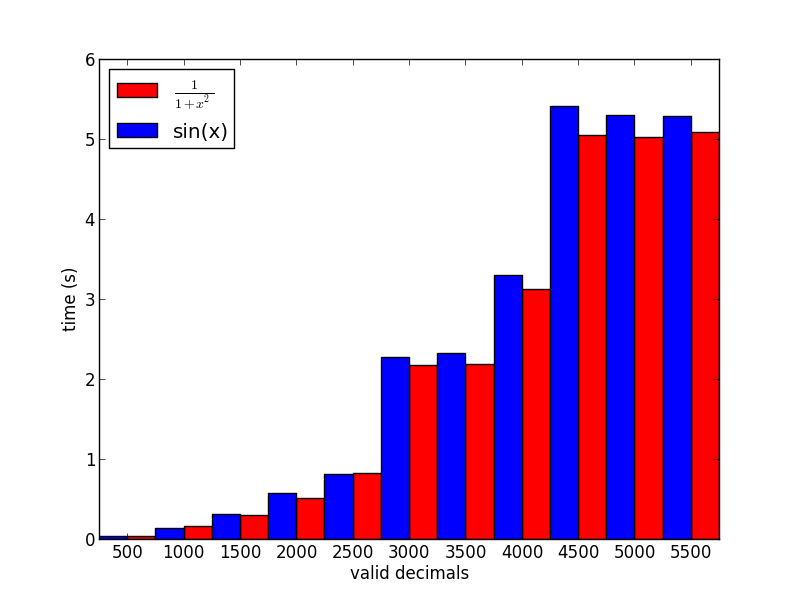
\includegraphics[width=0.5\textwidth]{img/analytic/ba_ana_dep_on_n_bar.png}
				\caption{running time evaluating \baana at fixed point $x=0.8$ depending on the desired number of valid digits}
				\label{fig:ba_ana dep on n}
			\end{figure}
			Running time Integration, Differentiation, Coefficient computation 
		\subsection{\anarect}
	\section{Applications}